\documentclass[9pt]{beamer}
\usetheme[progressstyle=movCircCnt]{PBEsimple}

\usepackage[T1]{fontenc}
\usepackage[utf8]{inputenc}
\usepackage[portuguese]{babel}
\usepackage{animate}
\usepackage{multicol}
\usepackage{amsfonts}
\usepackage{multirow}
\usepackage{array,booktabs}
\newcommand{\PR}[1]{\ensuremath{\left[#1\right]}}
\newcommand{\PC}[1]{\ensuremath{\left(#1\right)}}
\newcommand{\chav}[1]{\ensuremath{\left\{#1\right\}}}

\title[Bioestatística]{\bf Bioestatística\\
\vspace{.3\baselineskip}}
\subtitle[]{\bf}

\date{ 09 de Março de 2017}
\author[Isolde Previdelli]{
  Isolde Previdelli\\
  \href{itsprevidelli@uem.br}{{\tt itsprevidelli@uem.br \\
isoldeprevidelli@gmail.com \\ \vspace{8mm} \tt \textbf{\LARGE{AULA 4 -
    Análise Bivariada}}}}
}
\institute[PBE/UEM]{}

% % % % % % % % % % % % % % % % % % % % % % % % % % % % % % % % % %

\begin{document}
% Página Título
{\pbebg
\begin{frame}[plain,noframenumbering]
  \titlepage
\end{frame}}

%%%%%%%%%%%%%%
\begin{frame}{Sumário}{}
\tableofcontents
\end{frame}
%%%%%%%%%%%%%%

\section{Análise Bivariada}
\subsection{Tabelas bivariadas}

\begin{frame}{Coeficientes Bivariados}{}

\begin{block}{blue}{Coeficientes - Estimativas pontuais}
\begin{itemize}

\item Covariância
\item Coeficiente de Contigência C
\item Correlação linear de \textit{Pearson}
\item Correlação por postos de \textit{Spearman}
\item Correlação por postos de \textit{Kendall}
\item Coeficiente de concordância de \textit{Kappa}

\end{itemize}
\end{block}
\end{frame}


%\subsection{Análise Bivariada}
\begin{frame}{Objetivos}{}

\indent
\begin{block}{blue}{Objetivo Geral}
\begin{itemize}
\item \small{Descrever o comportamento de uma variável resposta em função de
outra (variável independente), isto é, resumir a variável resposta na
presença de outra.}
\end{itemize}
\end{block}



\begin{block}{blue}{Objetivos específicos}
\begin{itemize}
\item \small{Construir tabelas de dupla entrada}
\item \small{Construção de gráficos}
  \begin{itemize}
    \item gráfico de dupla barras
    \item diagrama de dispersão
    \item diagrama de caixas ou boxplot
  \end{itemize}
\end{itemize}
\end{block}
\end{frame}



\subsection{Tabela de contingência}
\begin{frame}{Tabelas de duas entradas ou contingência}{}

\indent
%\begin{block}{blue}{Variável quantitativa}
\begin{itemize}
\item A ocorrência simultânea de duas variáveis qualitativas são
  dispostas em tabela.
\item Coeficiente de Contingência C.
\end{itemize}
\textbf{Exemplo:} Deseja-se analisar o comportamento conjunto das
variáveis tipo de parto e tipo de hospital, usando uma amostra de 200
pacientes de Hospitais públicos e privados.
\begin{table}[!htb]
\centering
%\caption{My caption}
%\label{my-label}
\begin{tabular}{llll}
\hline
\multicolumn{1}{c}{\multirow{2}{*}{Hospital}} & \multicolumn{2}{c}{Parto} & \multicolumn{1}{c}{\multirow{2}{*}{Total}} \\ \cline{2-3}
\multicolumn{1}{c}{}                          & Natural    & Cesariano    & \multicolumn{1}{c}{}                       \\ \hline
Público                                       & 95         & 25           & 120                                        \\
Privado                                       & 35         & 45           & 80                                         \\ \hline
Total                                         & 130        & 70           & 200                                        \\ \hline
\end{tabular}
\end{table}
%\end{block}
\end{frame}


\subsection{Gráfico de barras}
\begin{frame}{Gráfico de barras duplas}{Exemplo}

Utilizado quando a variável resposta e a variável independente são
qualitativas. A altura da  barra representa freqüência da ocorrência
simultânea das duas categorias,  das  variáveis qualitativas.

\begin{figure}[!htb]
    \centering
    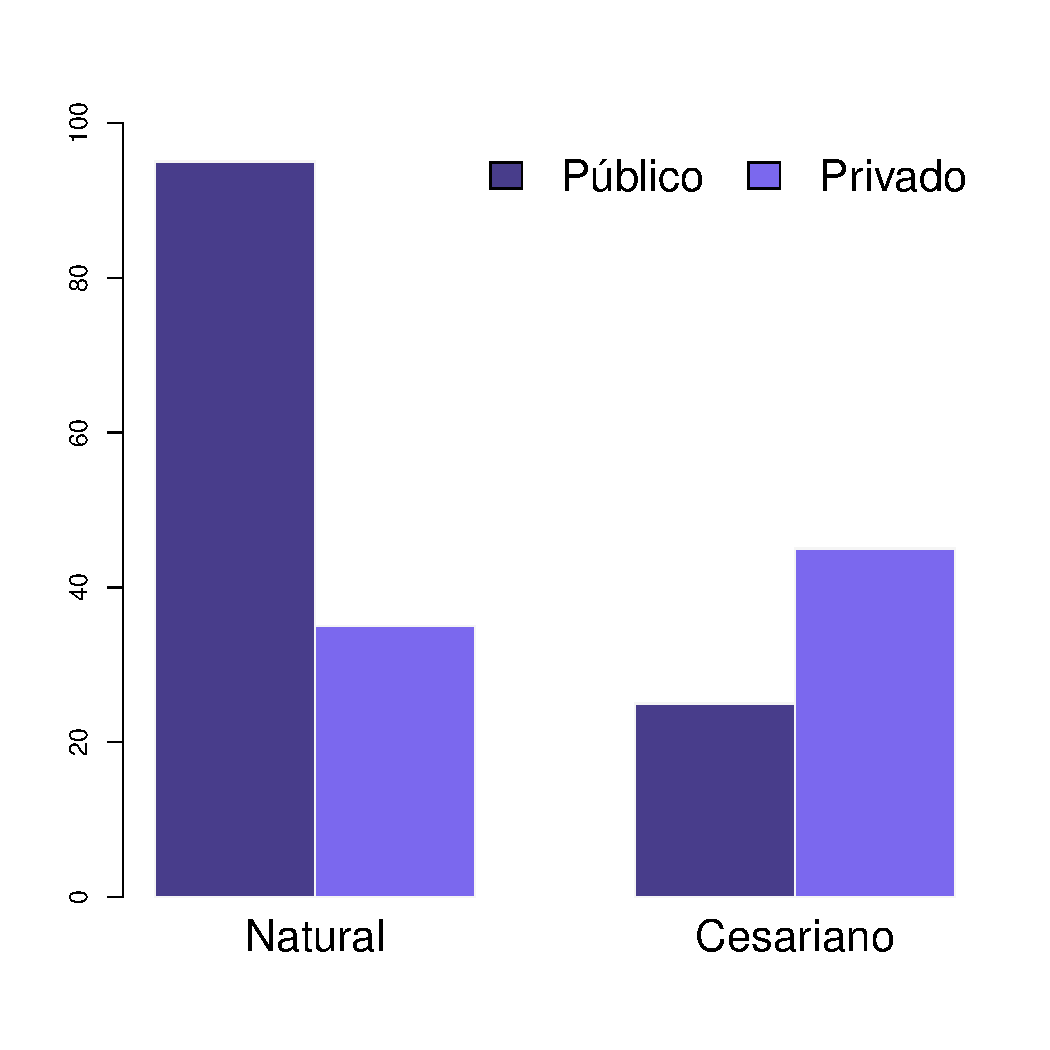
\includegraphics[scale=0.375]{barplot.pdf}
  \end{figure}

\end{frame}

\subsection{Coeficiente de Contingência C}
\begin{frame}{Coeficiente de contingência C}{}
%\begin{block}{red}{Covariância}
\begin{itemize}
\item É uma medida de associação entre duas variáveis em escala nomimal
%\item Independe de como as categorias das variáveis se dispõemnas linhas
%  e colunas da tabela de contingência
\item É um coeficiente de correlação não-paramétrico
\end{itemize}

\begin{itemize}
\item O cálculo do coeficiente de contingência é feito pela expressão abaixo:
\end{itemize}
$$
C = \sqrt{\frac{\displaystyle{\chi^2}}{\chi^2+n}}
$$
%\end{block}
em que $\chi^2 = \displaystyle{\sum_i \sum_j} =
\frac{\displaystyle{(O_{ij}-E_{ij})^2}}{E_{ij}}$

\begin{itemize}
 \item $O_{ij} =$ frequência onservada
 \item  $E_{ij} =$ frequência esperada, $E_{ij} = \frac{n_{i.}*n_{.j}}{n}$
\end{itemize}


em que
\begin{itemize}
 \item $n_{.j} = $ totais marginais(colunas)
 \item  $n_{i.} = $ totais marginais(linhas)
\end{itemize}

\end{frame}


\subsection{Diagrama de caixas - Boxplot}
\begin{frame}{Boxplot}{}
\begin{itemize}
\item Em uma investigação dos fatores de risco para as
    doenças cardiovasculares, os níveis séricos de cotinina - produto
    metabólico da nicotina - foram registrados para um grupo de
    fumantes e um grupo de não-fumantes.
\end{itemize}

\begin{figure}[!htb]
    \centering
    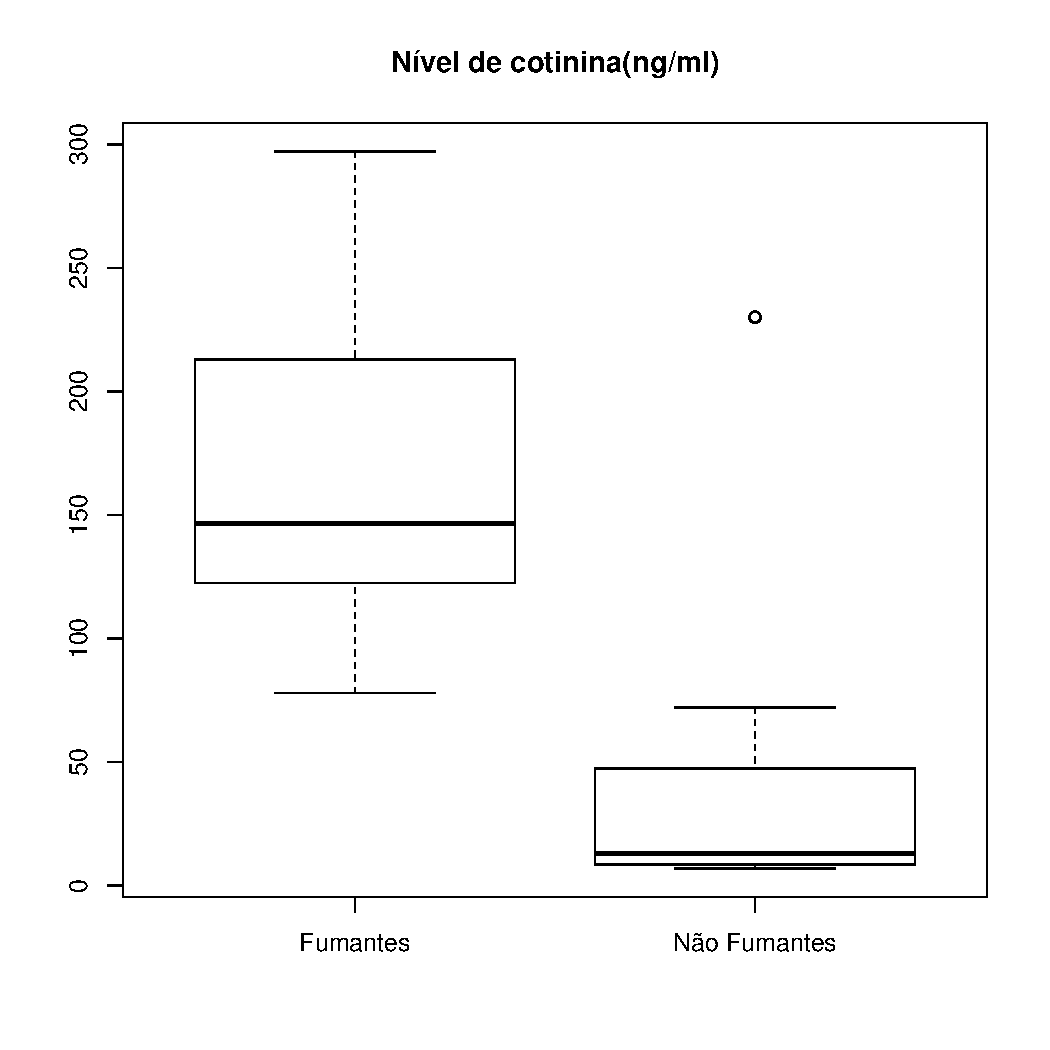
\includegraphics[scale=0.375]{boxplot.pdf}
  \end{figure}
\end{frame}


\subsection{Variáveis quantitativas}
\begin{frame}{Duas variáveis quantitativas}{}
\begin{block}{red}{Covariância e Coeficientes de correlação linear}
\begin{itemize}
\item Primeiro calcula-se a covariância
\item Coeficiente de correlação linear de \textit{Pearson}
  \begin{itemize}
    \item Paramétrico, dados emparelhados (x,y) independentes
   \end{itemize}

\end{itemize}

\begin{itemize}
\item Coeficiente de correlação por postos de \textit{Spearman}
  \begin{itemize}
    \item Não-Paramétrico, dados emparelhados (x,y) independentes, mas
      geralmente ordinais
   \end{itemize}

\item Coeficiente de correlação por postos de \textit{Kendall}
    \begin{itemize}
    \item Não-Paramétrico, útil para o mesmo tipo de dados ao qual se
      aplica
correlação de Spearman
   \end{itemize}

\end{itemize}
\end{block}

\end{frame}

\subsection{Covariância}
\begin{frame}{Covariância}{}
%\begin{block}{red}{Covariância}
\begin{itemize}
\item A covariância mede a relação linear entre duas variáveis
\item A covariância dá uma ideia da dispersão dos valores da variável bidimensional
\item A covariância não é padronizada
\end{itemize}

\begin{itemize}
\item O cálculo da covariância é feito pela expressão abaixo:
\end{itemize}
$$
Cov(x,y) = \frac{\displaystyle{\sum_{i=1}^n}(x_i-\bar{x})(y_i-\bar{y})}{n-1}
$$
%\end{block}
\end{frame}



\subsection{Correlação linear de Pearson}
\begin{frame}{Coeficiente de correlação linear de Pearson}{}
\begin{block}{red}{Suposições}
\begin{itemize}
\item A amostra de Dados Emparelhados (x,y) é independente.
\item Os pares de dados (x,y) têm distribuição Normal bivariada

\end{itemize}
\end{block}

\begin{block}{blue}{Para que serve?}
\begin{itemize}
\item Mede o grau de relacionamento linear entre os valores emparelhados
  x e y em uma amostra.
\item Utilizaremos o coeficiente de correlação linear para detectar
  padrões lineares.
\end{itemize}
\end{block}

\end{frame}


\begin{frame}{Coeficiente de correlação linear de Pearson}{}
\begin{block}{blue}{}
\begin{itemize}
\item Para verificar se exite correlação linear positiva, negativa ou
  inexistente entre duas variáveis quantitativas aplicam-se:
\begin{itemize}
  \item Gráfico: Diagrama de dispersão.
\end{itemize}

\item Coeficiente de correlação linear:
\begin{itemize}
  \item Correlação amostral é denotada pela letra "r";
    \item r - estimador;
      \item $\rho$ - parâmetro.
\end{itemize}

\end{itemize}
\end{block}
\end{frame}


\begin{frame}{Coeficiente de correlação linear de Pearson}{}

Para verificar o grau de relacionamento linear entre os valores
emparelhados x e y em uma amostra e verificar se existe correlação
linear positiva, negativa ou inexistência de correlação calcula-se:

$$
r = \frac{\displaystyle{ \sum_{i=1}^n} (x_i- \bar{x})(y_i -\bar{y})}{
\sqrt{\displaystyle{\sum_{i=1}^n} (x_i- \bar{x})^2 \sum_i (y_i-\bar{y})^2}}
$$
Ou ainda,
$$
r = \frac{Cov(x,y)}{s_{x} s_{y}}
$$

\begin{itemize}
\item Estatística $r$:
  \begin{itemize}
    \item é adimensional
      \item indicao grau de correlação entre duas amostras independentes
        \item varia de $-1$ a $1$
          \item se "r" for zero, não há relação linear entre as variáveis
  \end{itemize}
\end{itemize}


\end{frame}


\subsection{Diagrama de dispersão}
\begin{frame}{Diagrama de dispersão}{}

\begin{figure}[!htb]
    \centering
    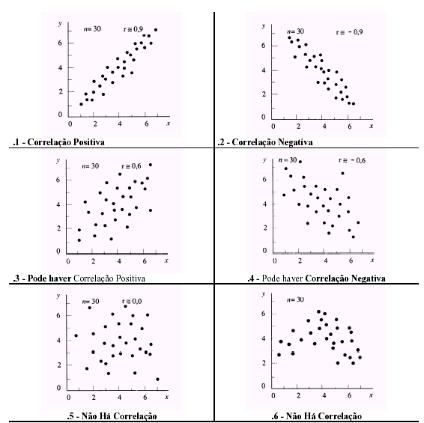
\includegraphics[scale=0.5]{disp.jpg}
  \end{figure}
\end{frame}



%\subsection{Diagrama de dispersão}
\begin{frame}{Correlação linear}{}

\begin{figure}[!htb]
    \centering
    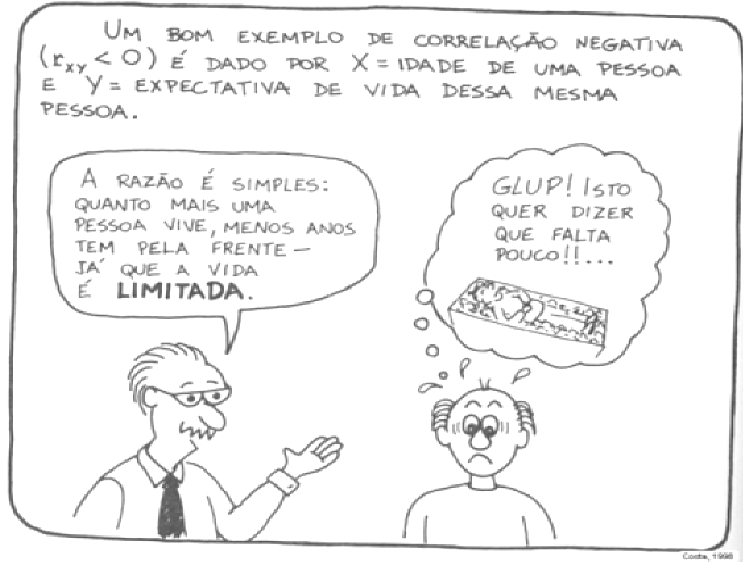
\includegraphics[scale=0.385]{fig.png}
  \end{figure}
\end{frame}


%\subsection{Diagrama de dispersão}
%\begin{frame}{Correlação linear}{}

%\begin{figure}[!htb]
 %   \centering
%    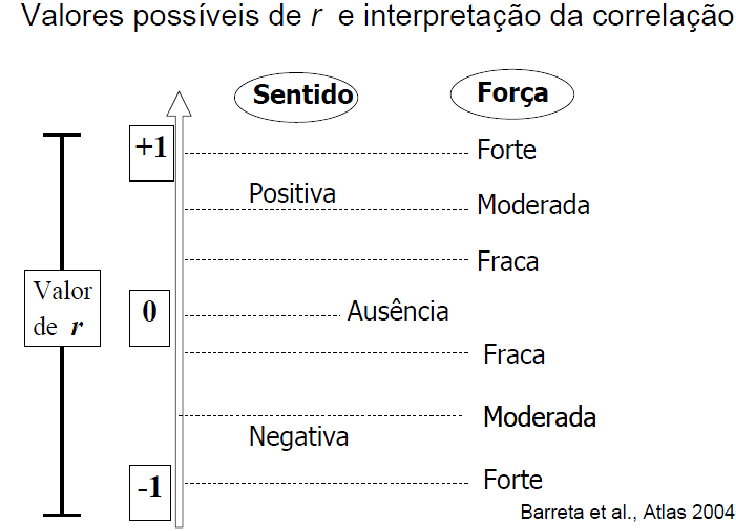
\includegraphics[scale=0.385]{fig2.png}
%  \end{figure}
%\end{frame}


\subsection{Correlação de Spearman}
\begin{frame}{Coeficiente de correlação por postos de Spearman}{}

É utilizado quando as duas variáveis, x e y:

\begin{itemize}
  \item São números com uma ordem de uma classificação
    \item Não apresentam distribuição conjunta normal  bivariada
\end{itemize}
Ou ainda

\begin{itemize}
  \item Nos casos dos dados não formarem uma nuvem comportada com pontos
    distantes dos demais, parece existir uma relação crescente ou
    decrescente num formato de curva
\item Desvantagens: Não leva em consideração os pesos amostrais
\end{itemize}
\end{frame}


\begin{frame}{Coeficiente de correlação por postos de Spearman}{}

Passos para calcular o coeficiente:

\begin{itemize}
  \item Ordenar todos os valores em cada amostra $(X_i, Y_i)$
    \item Atribuir números de ordem (atribuindo o número de ordem médio
      quando há empate) para cada amostra $Posto_{X_i}$ e $Posto_{Y_i}$
\end{itemize}


$$
r_{s} = 1- \frac{\displaystyle{6\sum_{i=1}^n d_{i}^2}}{(n^3-n)}
$$

 em que $d_i = X_i - Y_i$

\end{frame}


\subsection{Correlação de Kendall}
\begin{frame}{Coeficiente de correlação por postos de Kendall}{}

Passos para calcular o coeficiente:

\begin{itemize}
  \item Primeiro reordenamos os valores de modo que aparecam a ordem
natural(1,2,3,..,n) para $X_i$
    \item Em seguida calculamos $S = \displaystyle{\sum_{i=1}^n S_i}$
\end{itemize}
Veja o exemplo abaixo sobre notas atribuídas por dois médicos a 4
imagens de ressonância magnética:

\begin{table}
\begin{tabular}{lcccc}
\hline
Imagens & d & c & a & b \\
\hline
Médico X & 1 & 2 & 3  & 4  \\
Médico Y & 2  & 4 & 3 & 1  \\
\hline
\end{tabular}
\end{table}

\end{frame}


\begin{frame}{Coeficiente de correlação por postos de Kendall}{}

\begin{itemize}
\item  $1^0$ escore do médico Y é 2 e os pares que podemos formar
  são:(2,4);(2,3) e (2,1). Para o par que possui $1^0$ valor $< 2^0$
valor atribuímos o valor 1 e em caso contrário -1. Nesse caso temos,
$S_1 = 1+1-1=1$
\item $2^0$ escore do médico Y é 4 e então $S_2= -3$
\item $3^0$ escore do médico Y é 3 e então $S_3= -1$
\end{itemize}
Assim $S=1-3-1=-3$\\
Então calculamos o grau de correlação:

$$
\tau = \frac{S}{\frac{1}{2}(n(n-1))}
$$
Portanto, $\tau = -0,5$
\end{frame}

\subsection{Kappa}
\begin{frame}{Estatística Kappa}{}

Útil para avaliar concordância entre observadores, avaliadores, etc.
\begin{itemize}
\item Observador é uma fonte de erro
\item Por exemplo, examinar um raio X ou realizar um exame físico
\item Em geral os dados são apresentados em uma tabela de contigência
  $SxS$
\item \textit{Kappa} não é indicado para tabelas $2 x 2$ (Neste caso
  usa-se McNemar)
\end{itemize}

Coeficiente de \textit{Kappa}:

$$
\hat{k} = \frac{\Pi_0 - \Pi_e}{1-\Pi_e}
$$
Sendo $\Pi_0 = \displaystyle{\sum_{i=1}^s p_{ii}}=\displaystyle{
\sum_{i=1}^s} = \frac{n_{ii}}{n}$, a probabilidade de concordância com, $p_{ii}$ a
probabilidade de um indivíduo ser classificado na categoria i por ambos
os observadores e ,

$
\Pi_{e}=\displaystyle{\sum_{i=1}^s(p_{i+})(p_{+i})} =
\displaystyle{\sum_{i=1}^s
\frac{n_{i+}n_{+i}}{n n}}
$

\small{($\hat{k}=1$, concordância perfeita, $\hat{k}=0$, discordância total)}
\end{frame}


\begin{frame}{Estatística Kappa}{Exemplo}

Exemplo(Giolo S.R., 2004): Concordância entre diagnóstico de dois
neurologistas.\\

Os dados abaixo se referem a classificação de pacientes com esclerose
múltipla, em 4 classes de diagnóstico, por dois neurologistas.

\begin{table}[!htb]
\centering
%\caption{My caption}
%\label{my-label}
\begin{tabular}{llllll}
\hline
\multicolumn{1}{c}{\multirow{2}{*}{Neurologista 2}} &
                                                      \multicolumn{4}{c}{Neurologista 1} & \multicolumn{1}{c}{\multirow{2}{*}{Totais}} \\
\multicolumn{1}{c}{}                                & 1 & 2 & 3  &
                                                                   \multicolumn{1}{l}{4}  & \multicolumn{1}{c}{} \\ \cline{1-6}
1                                                     & 38                      & 5                       & 0                       & 1                       & 44                                           \\
2                                                     & 33                      & 11                      & 3                       & 0                       & 47                                           \\
3                                                     & 10                      & 14                      & 5                       & 6                       & 35                                           \\
4                                                     & 3                       & 7                       & 3                       & 10                      & 23                                           \\ \hline
\multicolumn{1}{l}{Totais}                          & \multicolumn{1}{l}{84} & \multicolumn{1}{l}{37} & \multicolumn{1}{l}{11} & \multicolumn{1}{l}{17} & \multicolumn{1}{l}{149}                     \\ \hline
\end{tabular}
\end{table}

Obteve-se:\\

$ \Pi_0 = (38+11+5+10)/149 = 0,4295$ \\
$\Pi_e = ((44*84)+(47*37)+(35*11)+(23*17))/149^2 = 0,2798$\\
\vspace{.55cm}
$\hat{k} = \displaystyle{\frac{0,4295 - 0,2798}{1-0,2798}} = 0,2079$\\
\vspace{.5cm}
\small{Tal resultado indica uma fraca concordância entre os neurologistas}
\end{frame}



%%%%%%%%%%%%%%%

{\pbebg
\begin{frame}[plain,noframenumbering]

\finalpage{\begin{figure}[!htb]
    \centering
    
\includegraphics[scale=0.43]{biv.png}
  \end{figure}
Obrigada!}

\end{frame}}
%%%%%%%%%%%%%%%%
\end{document}